\chapter{Entorno y plataforma de desarrollo}
\label{cap:entorno}

En este capítulo se describen los elementos que componen el sistema. El desarrollo del algoritmo no se limita únicamente a una implementación independiente a la que se somete a pruebas sintéticas para ver que se comporta según lo esperado, sino que se ha integrado dentro de un sistema robótico completo y funcional. Para poder hacer esto, es necesario adquirir una serie de conocimientos de todo el entorno de este sistema. Si bien no es necesario que este conocimiento sea exhaustivo y se tengan que conocer absolutamente todos los detalles, sí que hay que tener una idea muy clara de la arquitectura y su funcionamiento. \\

A continuación se explican los distintos componentes que se han utilizado para elaborar y probar el algoritmo. Se mostrará la plataforma robótica con la que se ha trabajado, se explicará la arquitectura del sistema robótico, las herramientas utilizadas y el algoritmo base sobre el que se sustenta la solución: el Filtro Extendido de Kalman. Para comenzar, en la figura \ref{fig:sistema}, se muestra un esquema general del funcionamiento del sistema y la conexión entre los distintos componentes. \\

\begin{figure} [h]
  \begin{center}
    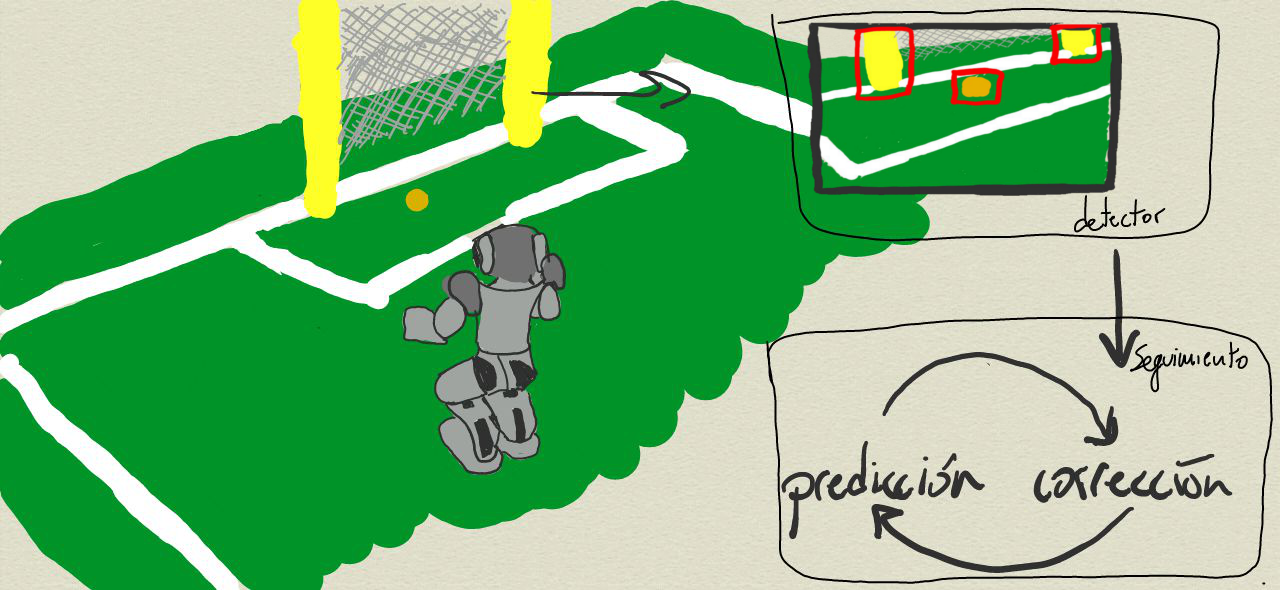
\includegraphics[width=15cm]{img/cap3/sistema}
  \end{center}
  \caption{Esquema general del funcionamiento del sistema}
  \label{fig:sistema}
\end{figure}

El robot capta las imágenes mediante una de las cámaras situadas en la cabeza. Normalmente se utiliza la cámara situada en la boca, porque está orientada hacia el suelo y facilita ver la pelota. La imagen es procesada por los detectores, que extraen los objetos interesantes que se encuentran en ella. En este caso serían los postes y la pelota. A continuación se procesan y filtran las observaciones para minimizar ruido, detectar posibles falsos positivos y fusionar con el resto de observaciones anteriores. El algoritmo desarrollado en este proyecto se encarga precisamente de esto. Su misión es obtener datos más robustos y fiables de una forma eficiente a partir de las observaciones de los detectores.\\

\section{Robot Nao}
\label{sec:robotnao}

 Nao es un robot humanoide de 58 cm de altura, figura \ref{fig:gradoslibertad}. Lo desarrolla la empresa francesa \textit{Aldebaran Robotics}\footnote{http://www.aldebaran-robotics.com/}. El proyecto de desarrollo del Nao nace en 2004. Al poco tiempo, en 2007, reemplaza al robot Aibo\footnote{http://es.wikipedia.org/wiki/Aibo}, creado por Sony, como el robot usado en la competición de la \textit{RoboCup Standard Platform League (SPL)}. En 2011 Aldebaran anuncia que van a lanzar el código fuente del controlador del Nao como software libre. Por el momento este robot es utilizado mayoritariamente en el ámbito académico, pero fuera de éste tiene muchos usos aún por descubrir. Las principales características del robot Nao son:

\begin{packed_item}
\item Gran cantidad de movimientos. El \textit{Nao RoboCup Edition}, que es la versión utilizada para la RoboCup y la que se utiliza en este proyecto, cuenta con 21 grados de libertad.
\item Detectores de presión en pies y manos, conocidos como FSR, \textit{Force Sensitive Resistors}. Este dispositivo tiene la capacidad de disminuir su resistencia cuando aumenta la fuerza aplicada sobre él. Suele utilizarse para el control de dispositivos electrónicos con el tacto.
\item Dos cámaras situadas en la cabeza con distintas zonas de visión. Una de ellas está situada en la frente del robot y apunta hacia el frente. La otra cámara esta situada en la boca del robot y tiene cierta inclinación hacia abajo. Los ángulos de visión de las cámaras no se solapan, en la figura \ref{fig:zonasvision} se puede ver hacia donde apunta cada cámara. Ambas tienen una resolución de 640x480 píxeles.
\item Cuatro sensores de ultrasonido colocados en el pecho del robot.
\item Un sensor inercial que mide la aceleración y la velocidad angular. Este sensor es muy útil en caso de caídas para detectarlas y actuar en consecuencia.
\item Interfaces de red Ethernet y WiFi que aportan conectividad al robot.
\item LEDs con distintos colores repartidos por el cuerpo del robot. Tiene uno en el botón de encendido y apagado del pecho del robot, un par en los ojos y varios en las orejas y pies.
\item Cuatro micrófonos colocados en la parte frontal, la parte posterior, al lado derecho y al lado izquierdo del robot.
\item Dos altavoces Hi-Fi en estéreo para reproducir sonidos colocados en la cabeza del robot.
\end{packed_item}

\begin{figure}[hbtp]
  \centering
  \subfloat[Sensores y actuadores del robot.]{
    \label{fig:gradoslibertad}
    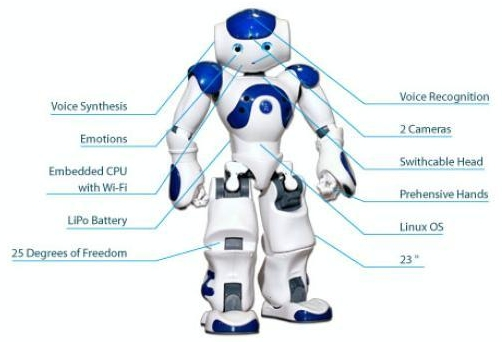
\includegraphics[width=9cm]{img/cap3/gradoslibertad}
  }
  \subfloat[Zonas de visión de cada una de las cámaras.]{
    \label{fig:zonasvision}
    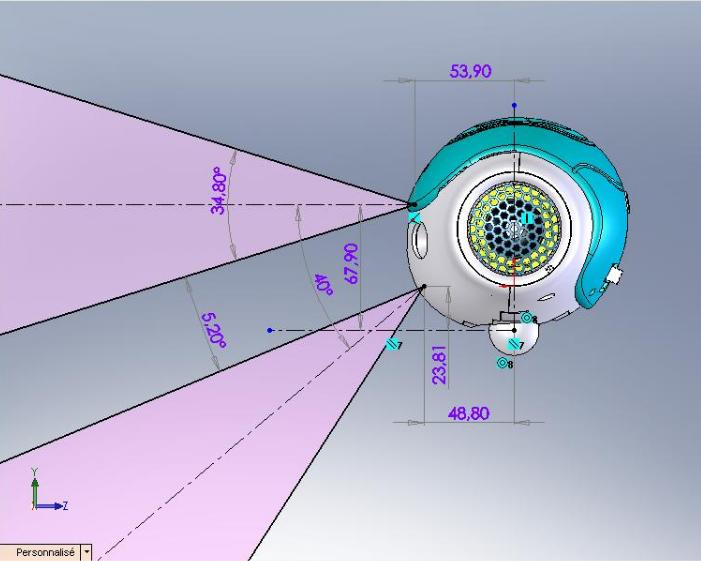
\includegraphics[width=6cm]{img/cap3/zonasvision}
  }
  \caption{El robot Nao.}
  \label{fig:robotnao}
\end{figure}

El robot dispone de un procesador x86 AMD Geode 500MHz y usa como sistema operativo Linux. Se alimenta de una batería recargable que le permite funcionar durante aproximadamente 45 minutos o durante quince minutos caminando sin parar. Este tiempo es suficiente para jugar una de las partes de un partido.\\

La apariencia de este robot es agradable y amigable. En los últimos años se está ampliando el ámbito de usos de este robot, que no se limita únicamente al fútbol robótico. Por ejemplo, hasta hace un año el Grupo de Robótica de la Universidad Rey Juan Carlos, estaba utilizando este robot en sesiones de Roboterapia con enfermos de Alzheimer en colaboración con la Fundación CIEN\footnote{http://www.fundacioncien.es}, \cite{Alzheimer2013} y \cite{RobotsEnTerapias2012}.

\section{NaoQi}
\label{sec:naoqi}

\textit{NaoQi} es un Framework, creado por Aldebaran Robotics, que permite desarrollar aplicaciones en C++ y Python en el Nao. Facilita el acceso a los sensores y actuadores del robot. Las aplicaciones creadas pueden ser ejecutadas directamente por el robot o remotamente en un ordenador.\\

Los ejecutables creados con este Framework se llaman \textit{broker}. Los \textit{broker} se ejecutan de forma independiente y se encuentran escuchando en una dirección IP y un puerto, por lo que pueden ser ejecutados en el propio robot, usando un compilador cruzado proporcionado por el Framework, o remotamente desde un ordenador. Un \textit{broker} esta formado por una serie de módulos que ofrecen distintas funcionalidades. Las funciones de estos módulos pueden ser llamadas desde otros módulos o incluso desde otros \textit{broker}.\\

\begin{figure} [h]
  \begin{center}
    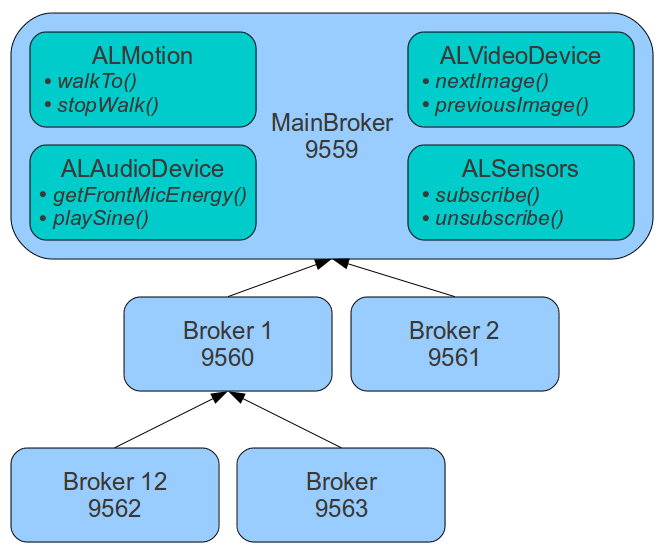
\includegraphics[width=9cm]{img/cap3/broker-naoqi}
  \end{center}
  \caption{Arquitectura de NaoQi modulada por medio de \textit{Brokers}.}
  \label{fig:broker-naoqi}
\end{figure}

En la figura \ref{fig:broker-naoqi} se puede ver un esquema de la arquitectura de \textit{NaoQi} modulada por medio de los \textit{broker}. El \textit{broker} más importante es el \textit{MainBroker} porque nos da acceso a los sensores y actuadores del robot. Cuando se desarrolla una aplicación para el robot con este Framework, se puede ejecutar a través de un \textit{broker} propio o como un módulo del \textit{MainBroker}; BICA se ejecuta de esta última manera. \textit{NaoQi} se utiliza para acceder a los sensores y actuadores de una manera más sencilla.\\

Los \textit{brokers} se organizan internamente en módulos. Cada uno de estos módulos aporta una funcionalidad concreta o permite acceder a sensores o actuadores del robot. Por ejemplo, \texttt{ALMotion} proporciona métodos que facilitan hacer que el robot se mueva; \texttt{ALAudioDevice} contiene otros módulos de \textit{NaoQi} que nos dan acceso a las entradas y salidas de audio; \texttt{ALVideoDevice} se encarga de proporcionar imágenes de las cámaras, y \texttt{ALSensors} es responsable de lanzar los eventos correspondientes cuando se pulsa un botón o se tocan las zonas táctiles de la cabeza o las manos.

\section{BICA}
\label{sec:bica}

BICA\footnote{http://www.robotica-urjc.es/index.php/Robocup}, \textit{Behavior-based Iterative Component Architecture}, es un software desarrollado en el grupo de Robótica de la Universidad Rey Juan Carlos, \cite{BICA2010} y \cite{BICA2013}. Se trata de una plataforma de desarrollo de software para el robot Nao. En la figura \ref{fig:bloques-bica} se puede ver la división en capas de la arquitectura de BICA.

\begin{figure} [hbtp]
  \begin{center}
    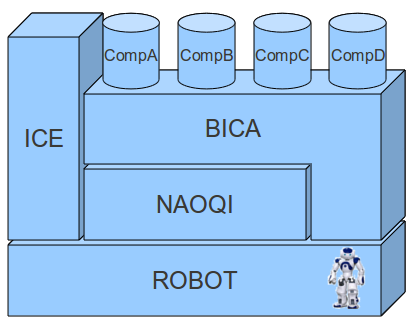
\includegraphics[width=7cm]{img/cap3/bloques-bica}
  \end{center}
  \caption{Arquitectura de BICA dividido en capas.}
  \label{fig:bloques-bica}
\end{figure}\

La unidad básica en la arquitectura de BICA es el \textit{componente}, representado en la figura \ref{fig:componente-bica}. La funcionalidad de los \textit{componentes} puede ser implementada mediante una máquina de estados o pueden ser controladores reactivos, es decir, que ejecutan al momento la acción requerida. Los \textit{componentes} pueden activarse o desactivarse. Un \textit{componente} activo ejecuta una tarea determinada de manera iterativa y con una frecuencia previamente fijada. Los \textit{componentes} que están activos iteran y consumen recursos. Los \textit{componentes} tienen una serie de métodos para modularlos y devuelven los resultados obtenidos.\\

\begin{figure} [hbtp]
  \begin{center}
    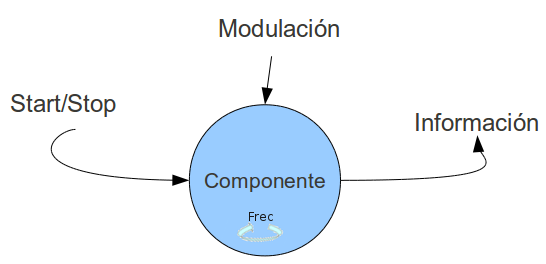
\includegraphics[width=9cm]{img/cap3/componente-bica}
  \end{center}
  \caption{Esquema de las entradas y salidas de un componente de BICA.}
  \label{fig:componente-bica}
\end{figure}

Para realizar tareas más complejas los \textit{componentes} pueden comunicarse entre sí. La arquitectura de BICA tiene una estructura jerárquica, tal y como se muestra en la figura \ref{fig:componentes-bica}. Cuando se activa el \textit{componente A}, éste activa los \textit{componentes D} y \textit{E}. A su vez, el componente \textit{D} activa los \textit{componentes G} y \textit{H}, y el \textit{componente E} activa los \textit{componentes H}, \textit{I} y \textit{J}. Un \textit{componente} puede ser activado por varios \textit{componentes}. Aunque sea llamado repetidas veces, éste se ejecutará a la frecuencia mínima que tenga configurada para evitar ciclos innecesarios y se ahorren recursos. Los \textit{componentes} de ''bajo nivel'', como los \textit{componentes G}, \textit{H}, \textit{I} y \textit{J}, se comunican directamente con el robot u obtienen la información mediante llamadas de \textit{NaoQi}.\\

\begin{figure} [hbtp]
  \begin{center}
    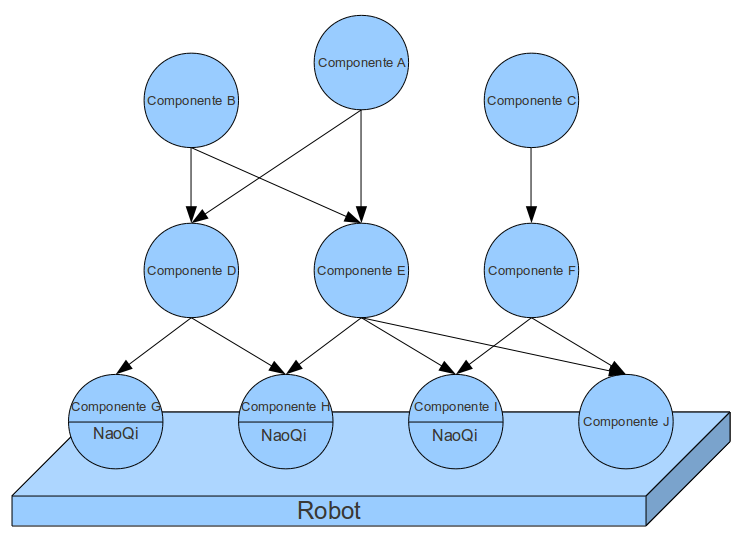
\includegraphics[width=9cm]{img/cap3/componentes-bica}
  \end{center}
  \caption{Jerarquía de componentes de BICA.}
  \label{fig:componentes-bica}
\end{figure}

A continuación se muestra un ejemplo en pseudocódigo muy básico del funcionamiento de los \textit{componentes}. Los \textit{componentes} tienen un par de métodos indispensables: \texttt{init()} y \texttt{step()}. Desde el método \texttt{init()} se inicializan los recursos necesarios para ejecutar el \textit{componente}. El método \texttt{step()} es el que activa el \textit{componente} y contiene toda su funcionalidad. Como el \textit{componente} se activa solamente cuando se llama a este método, no es necesario ningún otro método para detener su ejecución. Todos los \textit{componentes} disponen de un método privado llamado \texttt{isTime2Run()} que modula la frecuencia a la que se ejecuta el \textit{componente}. Si aún no tiene que ejecutarse el \textit{componente}, el método devuelve \texttt{false} y no se ejecuta ninguna instrucción del \textit{componente}.

\begin{lstlisting}[style=C]
void step() {
  // Ejecucion en cascada de los componentes de los que se
  // obtienen informacion.
  cp1->step();
  cp2->step();

  if (isTime2Run()) {
    // Recoger datos de los componentes perceptivos.

    // Iteracion genuina

    // Poner a disposicion del resto de componentes los datos
    // calculados y/o se modulan los componentes actuadores.
  }

  // Ejecucion en cascada de los componentes que se han
  // modulado o requieran ser ejecutados por su actuacion.
  ca1->step();
  ca2->step();
}
\end{lstlisting}

Al inicio del método \texttt{step()} se llama a los \textit{componentes} perceptivos, que son aquellos que devuelven datos, de los que depende el \textit{componente}. Si es el momento de que se ejecute el \textit{componente}, el método \texttt{isTime2Run()} devuelve \textit{true} y se ejecutan las instrucciones dentro de la estructura \textit{if}. Básicamente, lo que se hace en esta estructura es procesar los datos devueltos por los \textit{componentes} perceptivos y generar nuevos datos. En caso de que el \textit{componente} genere una respuesta, se modulan los \textit{componentes} actuadores, aquellos que generan una respuesta en el robot o procesan los datos que acabamos de crear. Por último, se llama al \texttt{step()} de éstos para que efectúen las acciones requeridas que acabamos de modular.\\

BICA está desarrollado en C++ y consiste en una arquitectura iterativa, formada por \textit{componentes} y basada en comportamientos. Proporciona un entorno de programación mono-hilo. Gracias a que se ejecuta en un sólo hilo nos evita las condiciones de carrera, un error muy frecuente y difícil de detectar en la programación concurrente.\\

Se ha escogido esta plataforma software por ser robusta y estar bastante probada. Ya ha sido utilizada en varios proyectos y es la plataforma utilizada en la RoboCup por el equipo de la Universidad. Además, dispone de varios \textit{componentes} que se pueden reutilizar. \\

Las comunicaciones con agentes externos se realizan a través del motor de comunicaciones de Internet, ICE, \textit{Internet Communications Engine}. Se trata de un \textit{middleware} de computación distribuida, orientado a objetos, multiplataforma y es desarrollado por la empresa \textit{ZeroC}\footnote{http://www.zeroc.com/}. Este \textit{middleware} proporciona una solución simple en el ámbito de las comunicaciones entre aplicaciones distribuidas en distintos servidores.\\

ICE dispone de una versión para sistemas embebidos, \textit{Ice-E}. Esta versión es un motor de comunicaciones más compacto diseñado para ejecutarse en entornos de recursos limitados, como teléfonos inteligentes o PDAs, por poner un par de ejemplos. Esta es la versión utilizada en el robot, ya que los recursos son bastante limitados y se necesita que el software corra lo más rápidamente posible. Gracias a ICE, BICA puede comunicarse con \textit{JManager} o con otros robots que usen BICA.

\subsection{Sistema de visión}
\label{subsec:sistemadevision}

La carga de trabajo del sistema de visión está distribuida en varios componentes. Básicamente el objetivo de este sistema es el de obtener, a partir de una imagen, los objetos interesantes que se encuentren en ella. Esta tarea de divide en varias subtareas más simples y abordables. El diagrama \ref{fig:visionsystem} muestra una secuencia de estos pasos.

\begin{figure} [h]
  \begin{center}
    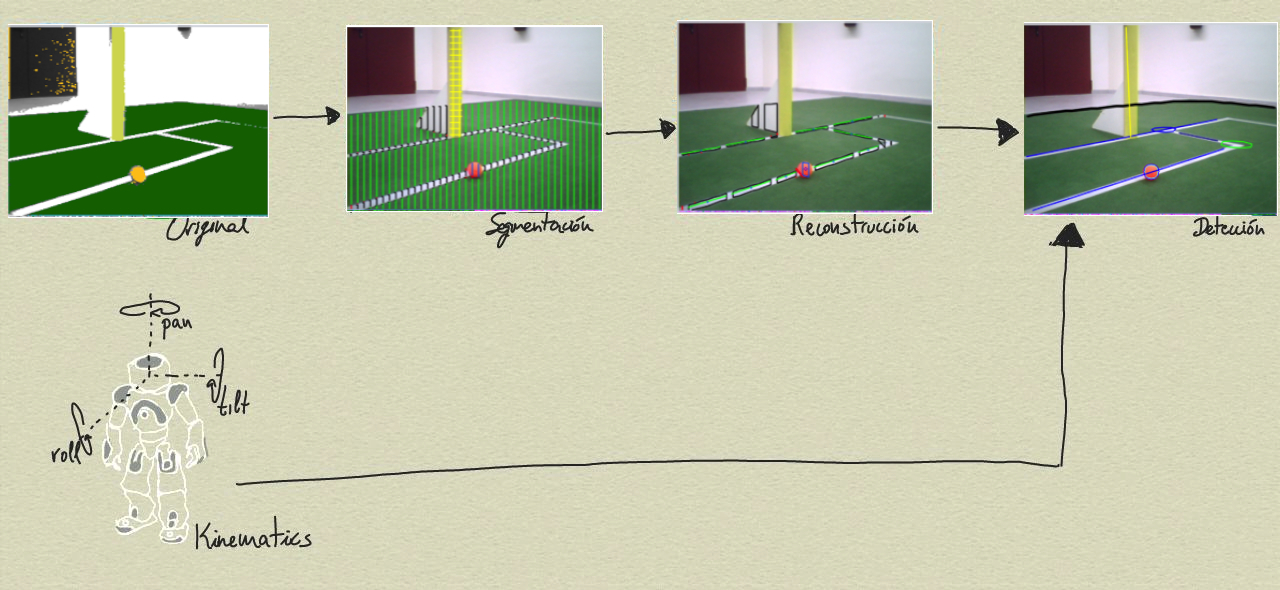
\includegraphics[width=15.5cm]{img/cap3/vision_system_real_images}
  \end{center}
  \caption{Esquema de funcionamiento del sistema de visión}
  \label{fig:visionsystem}
\end{figure}

En el momento en el que se obtiene una imagen se calculan lo que en el diagrama se ha etiquetado como \textit{kinematics}, en referencia al cálculo de los parámetros cinemáticos del robot. Se calcula la posición relativa de la cámara respecto del centro del robot. La cámara cuenta con tres grados de libertad: \textit{pan}, \textit{tilt}, \textit{roll}. Cada uno de estas medidas se corresponde con uno de los ejes del espacio tridimensional, en la figura \ref{fig:visionsystem} se puede ver a cuál corresponde cada uno de ellos. A partir de estos valores se averigua la matriz de traslación y rotación de la cámara, lo que nos permite transformar píxeles de la imagen 2D a puntos del entorno en 3D y viceversa. \\

Al mismo tiempo se procesa la imagen para extraer las características más interesantes de esta. Analizar imágenes es un proceso muy costoso que se repite muchas veces por segundo. Es primordial utilizar algoritmos rápidos y eficaces para que el robot pueda responder rápidamente a los estímulos. El algoritmo utilizado en BICA se conoce coloquialmente como \textit{rastrillado} de la imagen. En el diagrama es el paso etiquetado como segmentación. En vez de analizar completamente la imagen, se analizan una serie de columnas de esta. La resolución es ajustable. Cuanta menor es la resolución mayor es la velocidad de ejecución del algoritmo a costa de perder precisión. El algoritmo actual consume aproximadamente unos 8 milisegundos en analizar la imagen. \\

Para simplificar las tareas de análisis de las imágenes, el entorno de la RoboCup presenta una serie de colores bien definidos: las porterías son amarillas o azules, la pelota es naranja, el campo es verde, etc. Esta configuración permite filtrar la imagen por colores. Esta operación, comparada con otras técnicas de análisis de la imagen más avanzadas, es bastante liviana computacionalmente. Esto no quiere decir que sea \textit{pan comido}. Los algoritmos de visión tienen que ser igualmente robustos, ya que cualquier cambio en la intensidad de la luz puede afectar el rendimiento y resultado de estos. \\

Una vez segmentada la imagen, hay que reconstruirla, paso etiquetado como reconstrucción. Para ello, se analizan todos los segmentos de la imagen y se conectan los que tengan una relación de proximidad, es decir, se conectan los segmentos que tengan el mismo color y se encuentren a la izquierda, derecha, arriba o abajo el uno del otro. Al unir varios segmentos se regenera la imagen con masas amorfas de colores o \textit{blobs}. En un entorno como la RoboCup se puede sacar mucha información solamente a partir de estos \textit{blobs}. Según la resolución escogida, este conjunto de manchas se asemejará en mayor o menor medida a la realidad. \\

La detección de objetos en la imagen se hace a partir de la imagen reconstruida. Se comprueba que el color del objeto sea el correcto y se valida la observación teniendo en cuenta el tamaño y la forma real de dicho objeto. Aparte de estas validaciones básicas, hay que tener cuidado con objetos que se encuentren fuera del terreno de juego, pero que puedan asemejarse a cualquier elemento utilizado en el partido de fútbol. Véase el ejemplo de la \textit{niña baliza}, figura \ref{fig:ninabaliza}. En ediciones anteriores de la RoboCup se utilizaban una serie de balizas para simplificar la autolocalización del robot dentro del campo. En un campeonato apareció una niña vestida con los mismos colores que la baliza. Un método para apaliar estos falsos positivos es utilizar una frontera visual que limite el espacio donde realizar la búsqueda de un objeto. La frontera visual dibujada en el paso de reconstrucción de la figura \ref{fig:visionsystem} es un ejemplo de ello. Sólo es aplicable a la detección de la pelota, no de las porterías. El espacio de búsqueda se limita, como mucho, a un radio de 6 metros alrededor del robot. Con esto se asegura que cualquier objeto fuera de este radio está fuera del terreno de juego y se ignora. \\

\begin{figure} [h]
  \begin{center}
    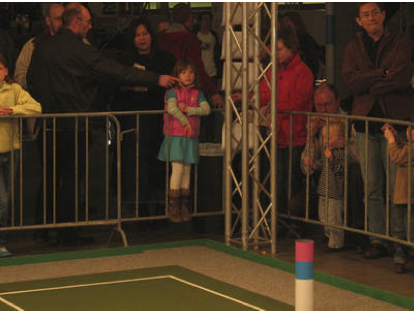
\includegraphics[]{img/cap3/nina_baliza}
  \end{center}
  \caption{La niña baliza}
  \label{fig:ninabaliza}
\end{figure}

Para calcular la posición de los objetos detectados en la imagen se utiliza la hipótesis suelo, figura \ref{fig:hipotesis-suelo}. De cada uno de los objetos se obtiene el píxel en el que intersecta con el suelo. A partir de este píxel -del cual se conoce la altura que es 0- la matriz de rotación y traslación de la cámara con respecto del robot calculada en el primer paso y una serie de cálculos geométricos, se calcula el punto 3D correspondiente con dicho píxel. Esta posición lleva un ruido asociado a ella. Todo junto es lo que se considera una observación, que es el dato de entrada del algoritmo desarrollado en este proyecto. \\

\begin{figure} [h]
  \begin{center}
    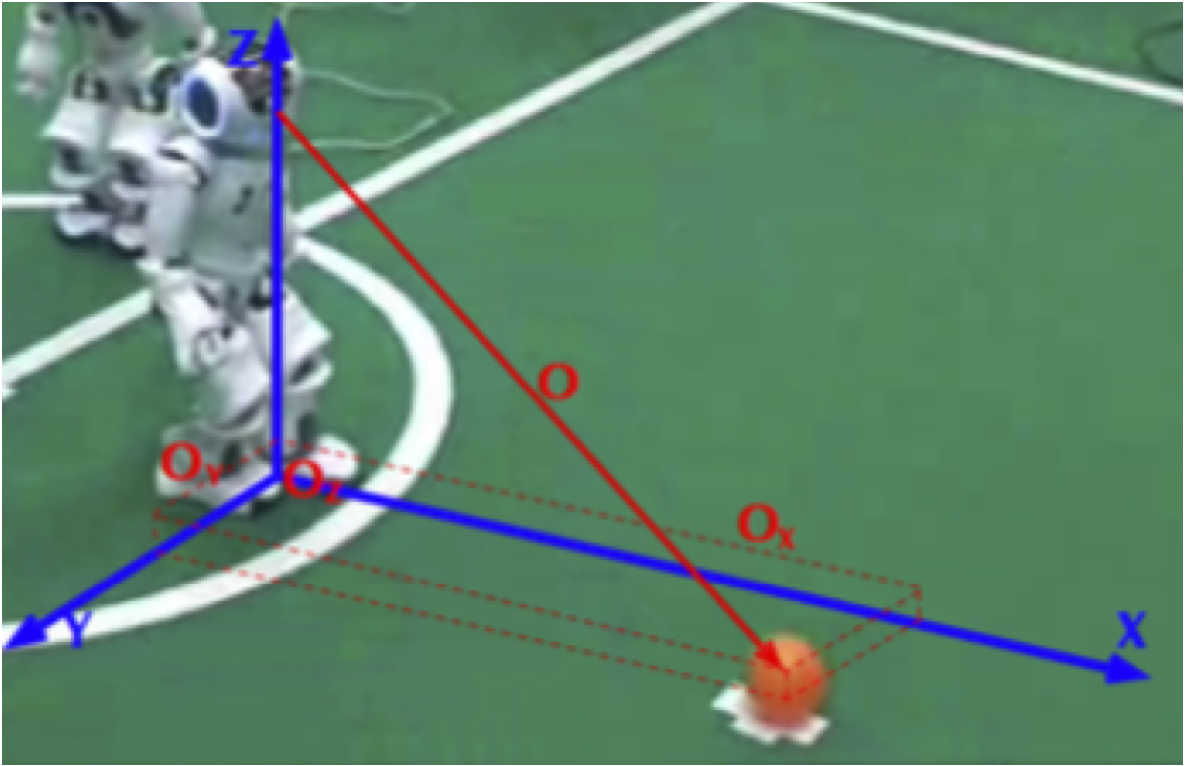
\includegraphics[width=9cm]{img/cap3/hipotesis_suelo}
  \end{center}
  \caption{Hipótesis suelo}
  \label{fig:hipotesis-suelo}
\end{figure}

\section{JManager}
\label{sec:jmanager}

JManager es una aplicación de escritorio desarrollada en Java que contiene herramientas para la monitorización, configuración y depuración de los algoritmos del robot. La figura \ref{fig:jmanagerscreenshot} está compuesta por un par de capturas de pantalla de esta aplicación. La aplicación JManager está organizada en varias pestañas, donde cada una proporciona una funcionalidad distinta. Una de estas funcionalidades es la activación y desactivación de los componentes disponibles en el robot, figura \ref{fig:jmanagerscreenshot02}. De igual manera se puede activar el modo de depuración y la interfaz gráfica propia de cada componente para modularlo y depurarlo. \\

\begin{figure}[h]
  \centering
  \subfloat[Administración de la conexión con el robot]{
    \label{fig:jmanagerscreenshot01}
    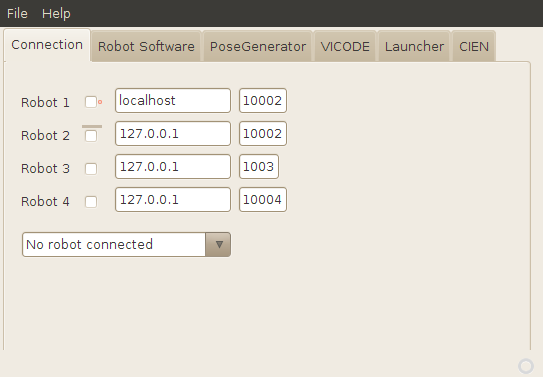
\includegraphics[width=6.5cm]{img/cap3/jmanager_screenshot01}
  }
  \subfloat[Administración de componentes]{
    \label{fig:jmanagerscreenshot02}
    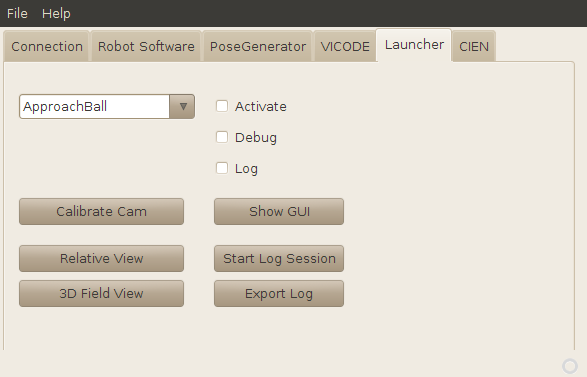
\includegraphics[width=7cm]{img/cap3/jmanager_screenshot02}
  }
  \caption{Capturas de pantalla de JManager}
  \label{fig:jmanagerscreenshot}
\end{figure}

Las conexiones con el robot se realizan a través de la red con ayuda de ICE. La figura \ref{fig:jmanager} es un esquema que representa la conexión entre JManager con la interfaz de ICE de cada componente. Todos los componentes que requieren de una conexión con el exterior, ya sea sólo para depuración o para comunicarse con otros agentes, implementan una de estas interfaces. En este caso la conexión se realiza desde el JManager, pero en caso de querer extender la funcionalidad con nuevas herramientas, sólo hay que implementar dichas interfaces. No es necesario tocar el código del robot. Esta capa de abstracción aporta una mayor independencia entre el código del robot y las herramientas de configuración y depuración.

\begin{figure} [h]
  \begin{center}
    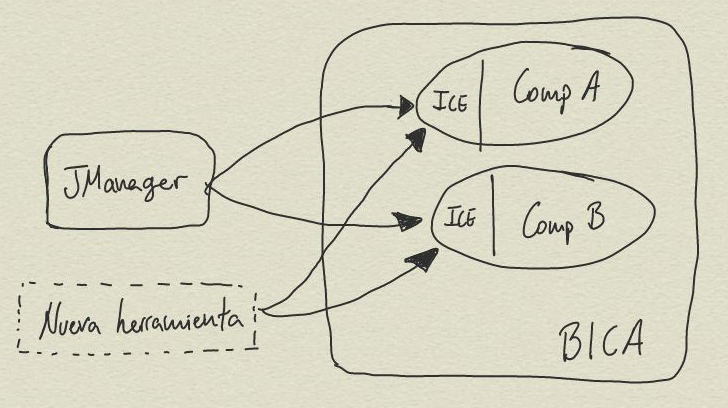
\includegraphics[width=12cm]{img/cap3/jmanager}
  \end{center}
  \caption{Conexión entre JManager y BICA.}
  \label{fig:jmanager}
\end{figure}

\subsection{Depurador de la memoria visual}
\label{subsec:depuradormemoriavisual}

Uno de los módulos que tiene JManager y que merece una mención especial es el depurador de la memoria visual, figura \ref{fig:depuradormemoriavisual}. El depurador consta de un espacio en la parte izquierda donde se pueden pintar distintas figuras geométricas representando los objetos que percibe el robot. La parte de la derecha se muestra información más detallada de algunos de los objetos más importantes del campo en una tabla, aunque en esta captura de pantalla no se está utilizando. \\

\begin{figure} [h]
  \begin{center}
    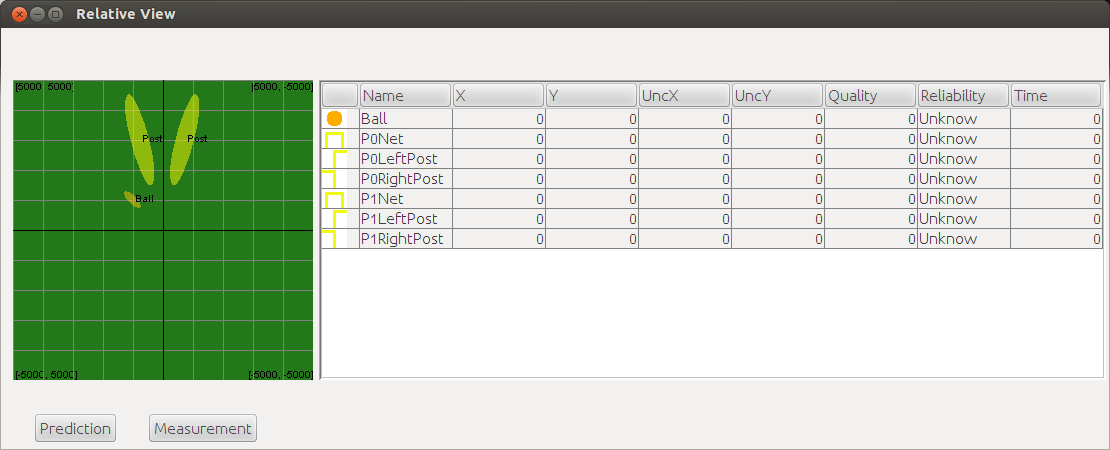
\includegraphics[width=15cm]{img/cap3/depurador_memoria_visual}
  \end{center}
  \caption{Captura de pantalla del depurador de memoria visual}
  \label{fig:depuradormemoriavisual}
\end{figure}

Los objetos que se muestran son un par de postes y la pelota. La incertidumbre de estos objetos se representa mediante una elipse. Cuanto menor es el tamaño de la elipse, menor es la incertidumbre. Esta representación visual es muy útil ya que de un solo vistazo se muestra mucha información. Por ejemplo, se puede ver claramente que los postes tienen más incertidumbre que la pelota. También se puede ver que, en general, se tiene mayor incertidumbre en cuanto a la distancia que en cuanto al ángulo con respecto del robot que se encuentran los objetos. Como la incertidumbre de las dos variables es distinta, la figura geométrica es una elipse. Si por el contrario la distancia y al ángulo tuviesen la misma incertidumbre, la figura sería un círculo. \\

El depurador se ejecuta en tiempo real y permite ver en todo momento en qué estado se encuentra la memoria de los objetos del robot: la posición en la que se encuentran y su incertidumbre. Esta herramienta es básica para la depuración y validación de los algoritmos de visión.

\section{Simulador}
\label{sec:simulador}

Los simuladores son herramientas que simulan un entorno real con todas sus propiedades físicas. Es una herramienta indispensable para el desarrollo de algoritmos complejos en robótica, ya que aumenta mucho el ritmo de trabajo. \\

El robot y los objetos simulados se definen mediante una serie de propiedades, como, por ejemplo, la forma, el color, la textura y la masa. También se simulan los sensores del robot, de manera que el robot sólo percibe lo que le llega a través de estos. Es importante que la simulación represente lo más fielmente posible la realidad para que los algoritmos desarrollados funcionen después en un robot real. \\

Para demostrar la importancia de los simuladores en la robótica, en la figura \ref{fig:darpavrc} se puede ver una par de imágenes de una competición que organiza el Departamento de Defensa de EE.UU.\footnote{http://www.darpa.mil/Our\_Work/TTO/Programs/DARPA\_Robotics\_Challenge.aspx} en el que se programa un robot humanoide, Atlas\footnote{http://es.wikipedia.org/wiki/Atlas\_(robot)},  para realizar una serie de tareas complejas tales como desplazarse por terrenos complejos, subirse y bajarse de un buggy, conducir el buggy con volante y pedales o enchufar una manguera a una boca de riego y abrir la válvula, que son solo algunas de ellas. Los ganadores de la competición reciben una importante suma de dinero, un robot Atlas y el derecho a participar en una competición similar a la simulada, pero con los robots reales. Y todo ello habiendo utilizado sólamente un simulador. \\

\begin{figure}[h]
  \centering
  \subfloat[Enchufando una manguera a una boca de riego]{
    \label{fig:atlasmanguera}
    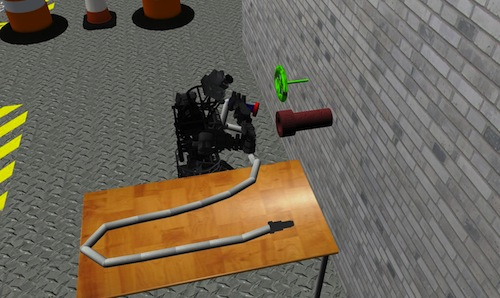
\includegraphics[width=7cm]{img/cap3/atlas_manguera}
  }
  \subfloat[Conduciendo un buggy]{
    \label{fig:atlasdriving}
    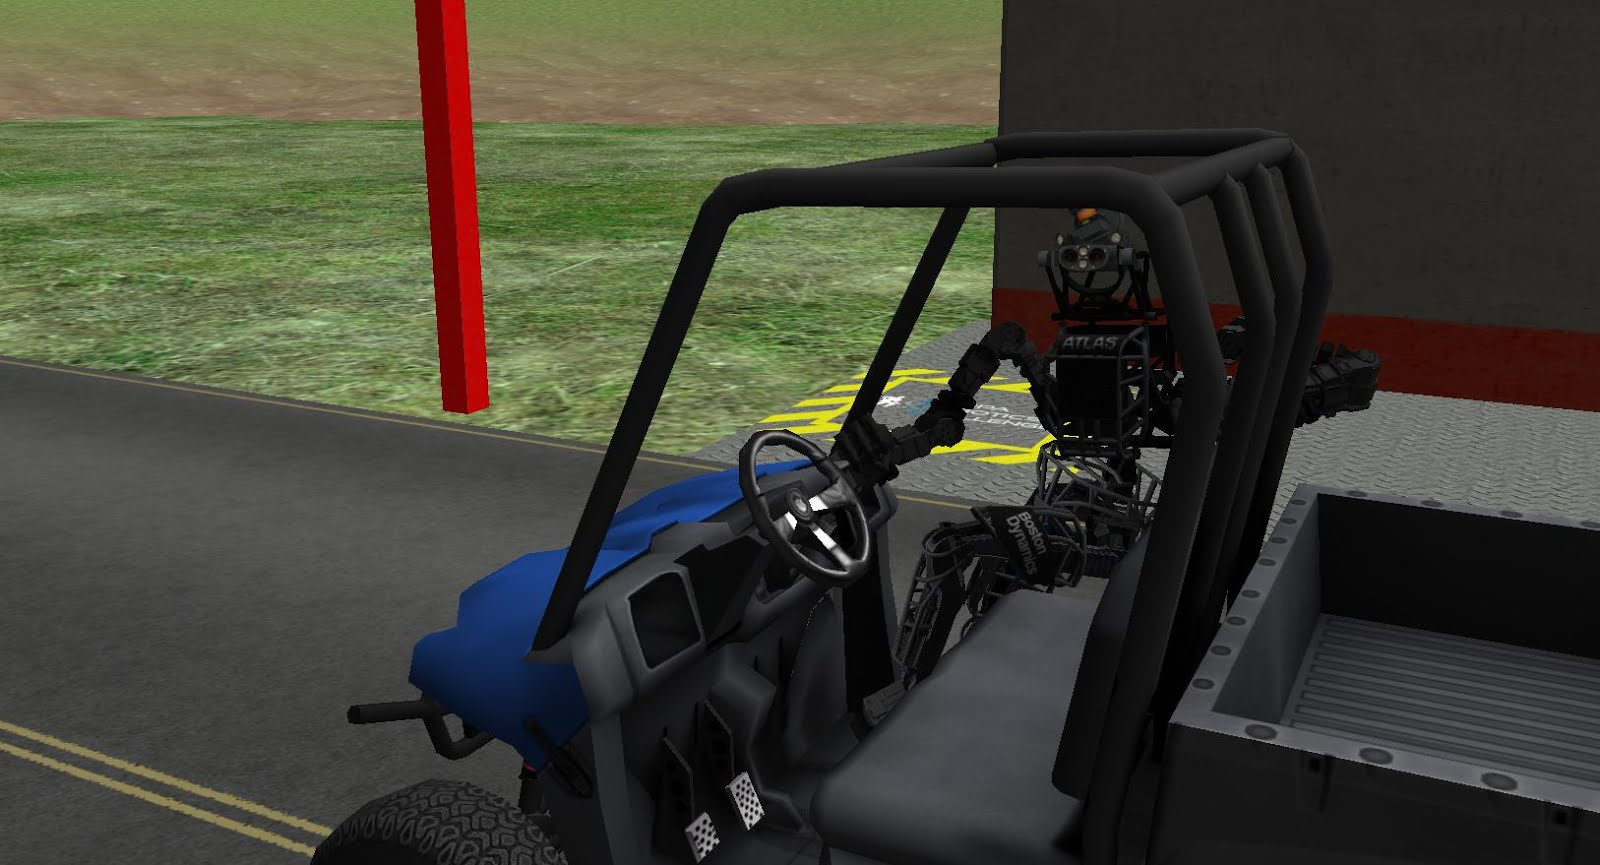
\includegraphics[width=7.7cm]{img/cap3/atlas_driving}
  }
  \caption{Robot Atlas en un par de pruebas de la DARPA VRC}
  \label{fig:darpavrc}
\end{figure}

Las pruebas de validación de este proyecto se han realizado en un escenario idéntico a un campo oficial de la RoboCup SPL. El algoritmo que se ejecuta es exactamente el mismo que luego se ejecuta en el robot real. La única diferencia es que la imagen procesada es una imagen del simulador en vez de ser una real. \\

\section{Estimación probabilística: Filtro Extendido de Kalman}
\label{sec:filtroextendidodekalman}

El Filtro de Kalman (KF) es un algoritmo de procesado de datos óptimo y recursivo. Este método fue descrito por Rudolf E. Kalman en 1958 para estimar los estados de un sistema estocástico. Estima el estado no observable de un sistema dinámico dado un conjunto de observaciones que proporcionan información acerca del estado en cada instante. Al ser recursivo no es necesario mantener los datos previos. Esta información se encuentra implícita en el estado, hecho que facilita en gran medida su implementación en sistemas de tiempo real. El algoritmo de Kalman estima los estados de manera óptima minimizando el índice del error cuadrático medio.\\

El KF solo es aplicable en sistemas lineales. Cuando se modela un entorno real los sistemas casi nunca son lineales, son más complejos. Por ejemplo, cuando un objeto rota alrededor del robot con una trayectoria circular, ésta no puede describirse como una transición lineal. El Filtro Extendido de Kalman (EKF) es la versión para sistemas no-lineales del KF. A costa de ampliar la familia de sistemas dinámicos el EKF pierde la optimalidad del algoritmo, aunque puede llegar a serlo si, tanto la transición del estado como la incorporación de las nuevas medidas, son lineales. Además, si la estimación inicial del estado es incorrecta o el proceso está mal modelado, el filtro puede diverger rápidamente. A pesar de estos inconvenientes, el EKF se considera el algoritmo \textit{por defecto} en sistemas de navegación y GPS.\\

El Filtro de Kalman representa la estimación de un estado en un instante de tiempo. En el período de tiempo $t$, esta estimación se representa por la media $s_t$ y la covarianza $P_t$. El cálculo del siguiente estado y la fase de corrección están dirigidas por las funciones no lineales $g$ y $h$, respectivamente:
\begin{equation}
s_t = g(u_t, s_{t-1}) + \epsilon_t
\end{equation}
\begin{equation}
z_t = h(s_t) + \delta_t
\end{equation}
donde $s_t$ y $s_{t-1}$ son vectores de estado, y $u_t$ es el vector de control en el tiempo $t$. Ambos vectores son verticales y tienen la forma
\begin{equation}
x_t = \begin{pmatrix}
      x_{1,t} \\ 
      x_{2,t} \\ 
      \vdots \\ 
      x_{n,t}
      \end{pmatrix}
\text{ y }
u_t = \begin{pmatrix}
      u_{1,t} \\ 
      u_{2,t} \\ 
      \vdots \\ 
      u_{m,t}
      \end{pmatrix}
\end{equation}

La idea que subyace en el EKF es la linealización. Existen muchas técnicas para linealizar funciones no lineales. EKF utiliza el método conocido como \textit{expansión de Taylor}. Este método construye una aproximación lineal de una función $g$ a partir del valor actual de $g$ y su pendiente. La pendiente se calcula con la derivada parcial de la función
\begin{equation}
g'(u_t, s_{t-1}) := \frac{\partial g(u_t, s_{t-1})}{\partial s_{t-1}}
\end{equation}

El estado de una sistema de Kalman normalmente tiene más de una dimensión. En estos casos en vez de la derivada simple se utiliza la matriz \textit{Jacobiana}. Si $f:\mathbb{R}^n \rightarrow \mathbb{R}^m$ es una función que va del espacio euclídeo $n$-dimensional a otro espacio euclídeo $m$-dimensional, las derivadas parciales de estas $m$ funciones se organizan en una matriz de tamaño de $m \times n$. \\
\begin{equation}
  J = 
  \begin{pmatrix}
    \frac{\delta f_1}{\delta x_1} & \cdots & \frac{\delta f_1}{\delta x_n} \\
    \vdots                        & \ddots &                        \vdots \\
    \frac{\delta f_m}{\delta x_1} & \cdots & \frac{\delta f_m}{\delta x_n} \\    
  \end{pmatrix}
\end{equation}

\subsection{El algoritmo EKF}

El algoritmo puede verse en la ecuación \ref{eq:ekf_algorithm}. El EKF representa la estimación en el tiempo $t$ de la media $s_t$ y la covarianza $P_t$. Los datos de entrada del filtro es la estimación en el tiempo $t-1$, que se representan como $s_{t-1}$ y $P_{t-1}$. Para actualizar estos parámetros, son necesarios los parámetros de control $u_t$ y las observaciones $z_t$. El dato de salida es la estimación en el tiempo $t$, que se representa por $s_t$ y $P_t$.
\begin{equation}
\label{eq:ekf_algorithm}
\begin{array}{ll}
1: & \large{\textbf{EKF}}(u_{t-1}, P_{t-1}, u_t, z_t) \\
2: & \bar{s_t} = g(s_{t-1}, u_t, 0) \\
3: & \bar{P_t} = A_t P_{t-1} A^T_t + W_t Q_t W^T_t \\
4: & K_t = \bar{P_t} H^T_t ( H_t \bar{P_t} H^T_t + V_t R_t V^T_t )^{-1} \\
5: & s_t = \bar{s_t} + K_t ( z_t - h( \bar{s_t}, 0 ) ) \\
6: & P_t = ( I - K_t H_t ) \bar{P_t} \\
7: & \mbox{return } s_t, P_t
\end{array}
\end{equation}

En las líneas 2 y 3, la estimación predecida $\bar{s}$ y $\bar{P}$ se calcula justo antes de incorporar la observación $z_t$. Esta estimación se obtiene incorporando los datos proporcionados por el vector de control $u_t$. Entre las líneas 4 y 6 se incorpora la observación $z_t$. La matriz de la \textit{Ganancia de Kalman} $K_t$ dice cuánto se confía en la nueva observación. El valor acotado por la llave se conoce como la \textit{innovación}.
\begin{equation}
4: s_t = \bar{s_t} + K_t \overbrace{( z_t - h( \bar{s_t}, 0 ) )}^\text{innovación}
\end{equation}
Es la diferencia entre la observación y la predicción. Un valor alto de la Ganancia de Kalman significa que se confía más en la observación que en la predicción, por lo que, el nuevo estado será más parecido a la observación que a la predicción. Si la ganancia de Kalman tiene un valor bajo, ocurre lo contrario. No se confía en la nueva observación y el nuevo estado será más cercano a la predicción que a la observación.\\

Las matrices $A$, $W$, $H$ y $V$ son las matrices Jacobianas obtenidas de la linealización del modelo del sistema. $A$ y $W$ son las jacobianas de $g()$ con respecto al estado $s$ y al ruido en la predicción del sistema $w$. $H$ y $V$ son las jacobianas con respecto a $s$ y al ruido de la observación $v$. Estas matrices se calculan a partir del estado actual $s$.

\subsection{Representación gráfica del EKF}
\label{subsec:representaciondelekf}

La figura \ref{fig:kalmangrafico} es una representación de cómo funciona el algoritmo de Kalman. Esta representación se hace sobre un modelo simple compuesto por una sola dimensión, pero permite ver y entender cómo funciona el algoritmo de Kalman muy fácilmente. \\

\begin{figure}
  \centering
  \begin{tabular}{cc}
  \subfloat[estimación inicial]{
    \label{fig:kalman1}
    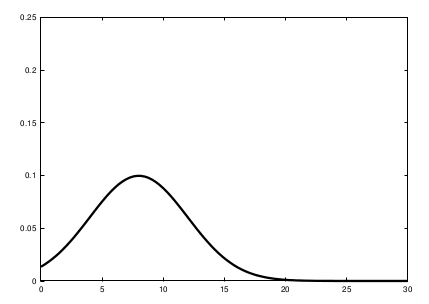
\includegraphics[width=0.45\textwidth]{img/cap3/kalman1}
  } &
  \subfloat[una observación (en negrita) con una incertidumbre asociada]{
    \label{fig:kalman2}
    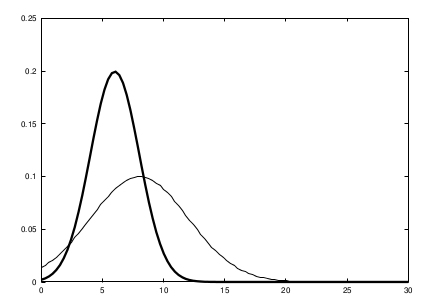
\includegraphics[width=0.45\textwidth]{img/cap3/kalman2}
  } \\
  \subfloat[estimación después de incorporar la observación a la estimación usando el algoritmo de un EKF]{
    \label{fig:kalman3}
    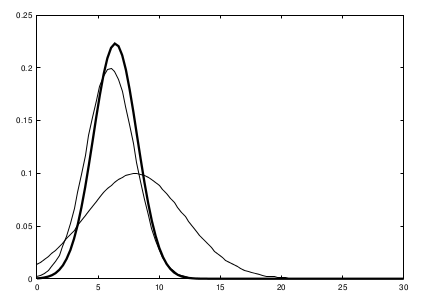
\includegraphics[width=0.45\textwidth]{img/cap3/kalman3}
  } &
  \subfloat[estimación después de un desplazamiento hacia la derecha, que introduce incertidumbre]{
    \label{fig:kalman4}
    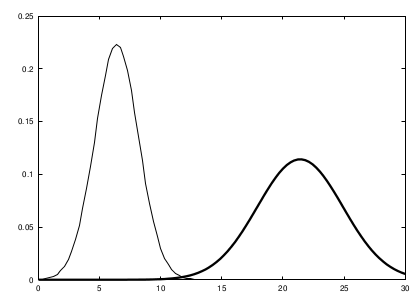
\includegraphics[width=0.45\textwidth]{img/cap3/kalman4}
  } \\
  \subfloat[una nueva observación con una incertidumbre asociada]{
    \label{fig:kalman5}
    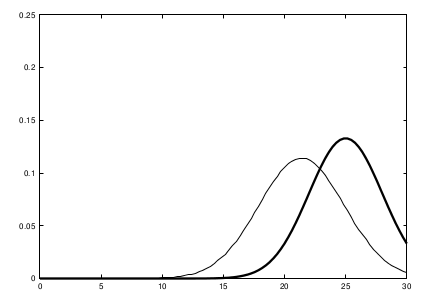
\includegraphics[width=0.45\textwidth]{img/cap3/kalman5}
  } &
  \subfloat[la incertidumbre asociada]{
    \label{fig:kalman6}
    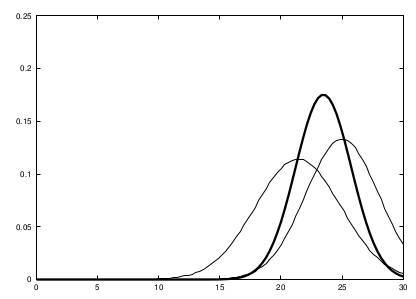
\includegraphics[width=0.45\textwidth]{img/cap3/kalman6}
  }
  \end{tabular}
  \caption{Ejemplo gráfico de un EKF}
  \label{fig:kalmangrafico}
\end{figure}

Se supone el caso de un robot que se mueve horizontalmente a lo largo de un raíl o sobre un eje. La estimación de la posición del robot se representa mediante una distribución normal. La estimación inicial del robot de donde está localizado se muestra en la figura \ref{fig:kalman1}. En la figura \ref{fig:kalman2} el robot obtiene una observación de uno de sus sensores, éste podría ser un GPS por ejemplo. Esta observación esta centrada en el pico de la gausiana representada con una línea de mayor grosor. El \textit{ancho} de esta gausiana es la incertidumbre asociada a dicha observación. La observación se incorpora al filtro y se obtiene una nueva estimación de la posición, pintada en negrita en la figura \ref{fig:kalman3}. El robot continúa desplazándose y después de un corto período de tiempo estima que su posición es la gausiana en negrita de la figura \ref{fig:kalman4}. Esta nueva estimación es más baja y ancha porque se introduce incertidumbre en la predicción de la nueva posición. Por último, en las figuras \ref{fig:kalman5} y \ref{fig:kalman6} se obtiene una nueva observación de la posición y se introduce al algoritmo para generar la nueva estimación.\\

A partir de la matriz de covarianza se puede dibujar una elipse que represente de forma gráfica el error en la muestra que representa dicha matriz. La elipse de error tiene el centro en las mismas coordenadas de la media del filtro de Kalman. Los atributos de la elipse se calculan por medio de los autovalores y autovectores. Los autovalores que se obtienen de la matriz de covarianza corresponden, cada uno de ellos, a uno de los semi-ejes de la elipse. Los autovectores nos indican la dirección de los semi-ejes. El ángulo de rotación de la elipse se calcula por medio de un simple cálculo trigonométrico a partir de uno de los autovectores. \\

Dada $A = \begin{pmatrix} a & b \\ c & d \end{pmatrix}$, que es una matriz $2x2$, $\lambda$ un número y $\hat{x}$ un vector $2x1$ con $\hat{x} \neq \hat{0}$, entonces $\lambda$ es un autovalor de $A$ y $\hat{x}$ es un autovector de $\lambda$ cuando

\begin{equation}
  A \hat{x} = \lambda \hat{x}
  \label{eq:eigenvalues}
\end{equation}

A partir de esta ecuación se pueden calcular los autovalores de la matriz de forma sencilla. Si se desarrolla un poco la ecuación anterior, tenemos
\begin{equation}
  \begin{split}
    A \hat{x} & = \lambda \hat{x} \\
    A \hat{x} - \lambda \hat{x} & = \hat{0} \\
    A \hat{x} - \lambda I \hat{x} & = \hat{0} \\
    \underbrace{( A - \lambda I )}_{\text{Soluciones no triviales} \iff det(A - \lambda I) = 0} \hat{x} & = \hat{0} 
  \end{split}
\end{equation}

El polinomio característico de la matriz es
\begin{equation}
\begin{split}
  p(\lambda) & = det(A - \lambda I) \\
             & = \begin{vmatrix} a - \lambda & b \\ c & d - \lambda \end{vmatrix} \\
             & = \lambda^2 - \underbrace{(a + d)}_{\text{diagonal}} \lambda + \underbrace{ad - bc}_{det(A)}
\end{split}
\end{equation}

Los valores obtenidos de resolver esta ecuación de segundo grado son los autovalores. Para cada uno de ellos hay que calcular su autovector correspondiente resolviendo la siguiente ecuación mediante el método que se prefiera
\begin{equation}
  \begin{pmatrix} a - \lambda & b \\ c & d - \lambda \end{pmatrix} \hat{x} = \hat{0}
\end{equation} \\

La figura \ref{fig:elipses} es una representación gráfica de las elipses de error donde se ve muy fácilmente lo que se acaba de explicar. La elipse representa el grado de incertidumbre que tiene un robot respecto a su propia localización. El robot comienza a desplazarse con una incertidumbre muy pequeña, el tamaño de la elipse es muy pequeño. Según avanza la incertidumbre crece gradualmente porque no tiene ninguna referencia visual que le ayude a verificar su posición. En el momento que divisa una baliza o \textit{landmark}, el robot es capaz de calcular su posición y la incertidumbre comienza a disminuir. En el momento que la pierde, otra vez vuelve a crecer la incertidumbre.

Esta representación es muy fácil e intuitiva de ver. De un sólo vistazo se sabe la posición del robot, o de un objeto, y su incertidumbre asociada. \\

\begin{figure} [h]
  \begin{center}
    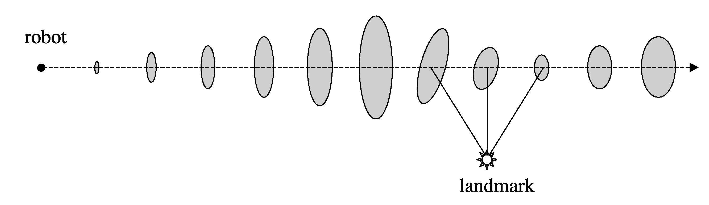
\includegraphics[width=15cm]{img/cap3/elipses}
  \end{center}
  \caption{Representación gráfica de las elipses de error}
  \label{fig:elipses}
\end{figure}

